\documentclass[14pt]{beamer}


\title[NST]{Neural Style Transfer}
\subtitle{NeuralArt - Stylize your Image}
\date{26 September 2020}

\usetheme{Madrid}
\usepackage{graphicx}

\begin{document}

\bgroup
\setbeamercolor{background canvas}{bg=black}
\begin{frame}[plain]{}
\end{frame}
\egroup


\begin{frame}
   \titlepage
\end{frame}

\begin{frame}
    \frametitle{About us}
    \begin{columns}
        \begin{column}{0.33\textwidth}
            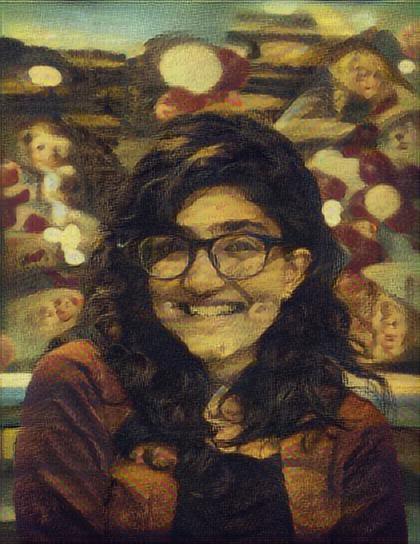
\includegraphics[width=30mm]{Avishi.jpg}\\
            \small Avishi Gupta\\
            
            \scriptsize Computer Science and\\Design undergraduate at\\IIIT Delhi
        \end{column}
        \begin{column}{0.33\textwidth}
            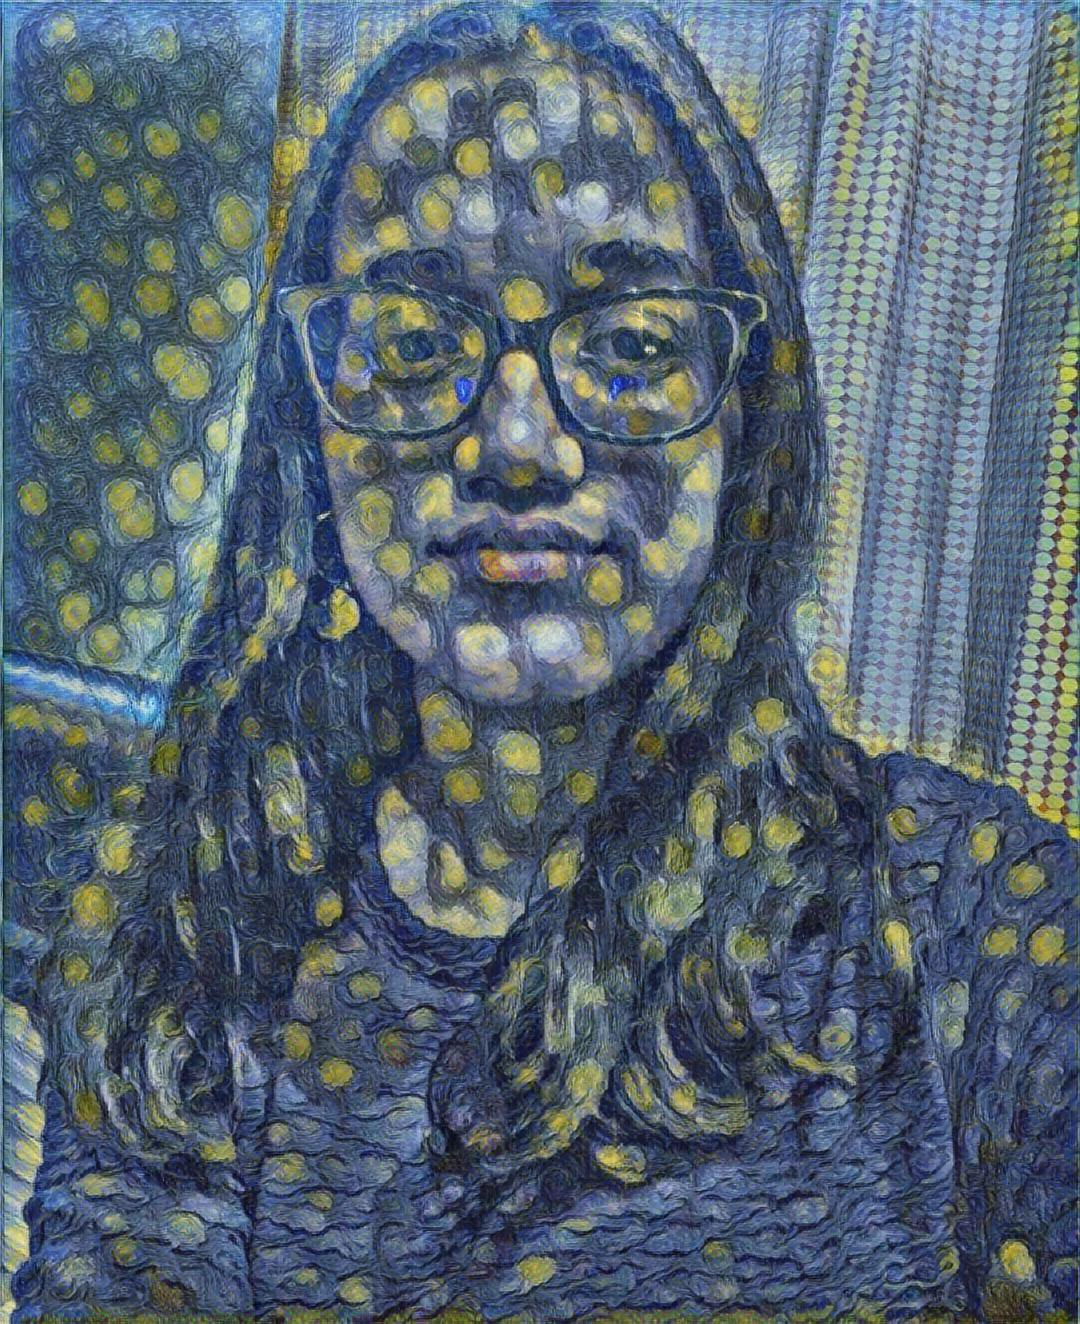
\includegraphics[width=32mm]{sshivangi.jpg}\\
            \small Shivangi Tomar\\
       
            \scriptsize Computer Science undergraduate at NIT Karnataka
        \end{column}
        \begin{column}{0.33\textwidth}
            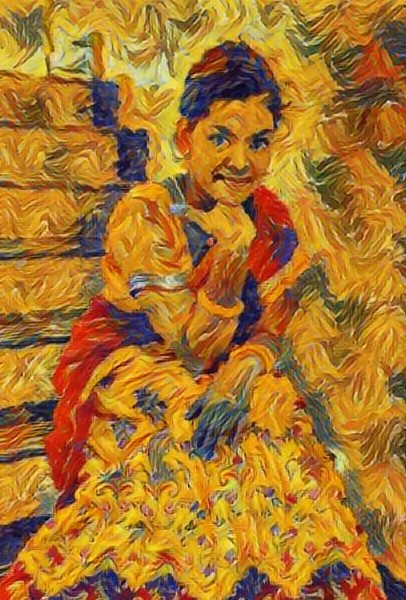
\includegraphics[width=27mm]{vnaaz.jpg}\\
            \small Vaseem Naazleen\\
            \scriptsize Computer Science undergraduate at VVIT, Andhra Pradesh
        \end{column}
    \end{columns}
\end{frame}

\begin{frame}
    \begin{center}
        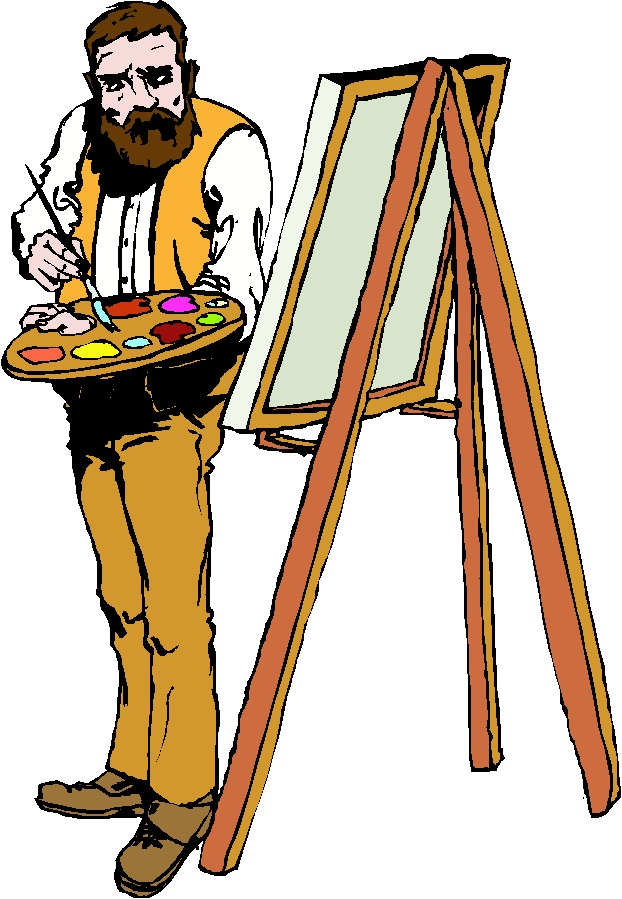
\includegraphics[width=50mm]{paints.jpg}
    \end{center}
\end{frame}

\begin{frame}
		\frametitle{Overview}
		Our project aims to stylize image by implementing A Neural Algorithm of Artistic Style paper by Leon A. Gatys, Alexander S. Ecker and Matthias Bethge. \\~\\

		https://arxiv.org/pdf/1508.06576.pdf
\end{frame}

\begin{frame}
    \frametitle{What is Neural Style Transfer?}
    \begin{center}
        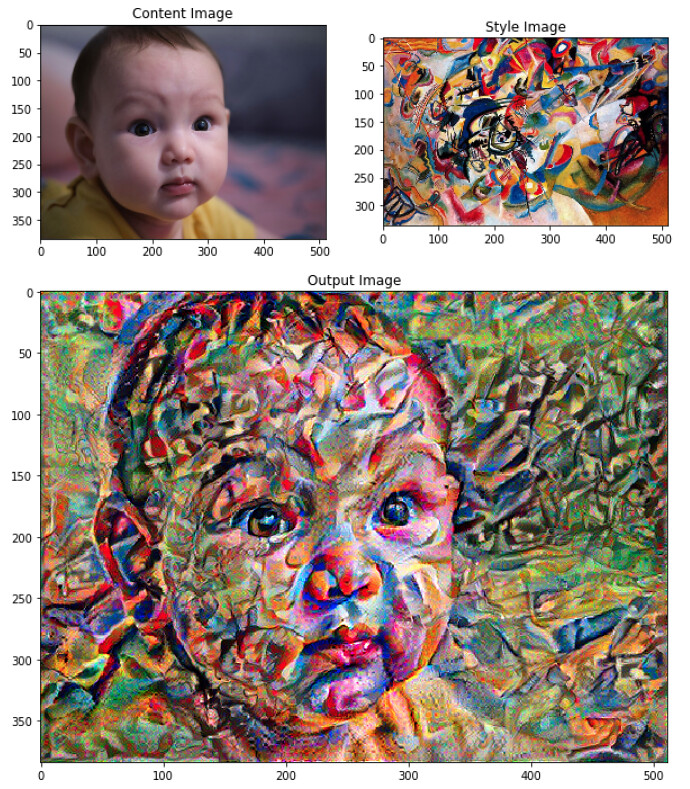
\includegraphics[width=60mm]{baby.jpeg}
    \end{center}
\end{frame}

\begin{frame}
		\frametitle{What is Neural Style Transfer?}
		\setbeamertemplate{itemize items}[ball]
		\begin{itemize}
            \item Neural Style Transfer is an optimization technique.
           \item Input:
		\begin{itemize}
		     \item Content image
		     \item Style reference image
		\end{itemize}
             \item Output:
		\begin{itemize}
             \item Stylized image: looks like the content image, but \say{painted} in the style of the style
        reference image.
        \end{itemize}
        \end{itemize}
\end{frame}

\begin{frame}
    \frametitle{What is Neural Style Transfer?}
    \begin{center}
        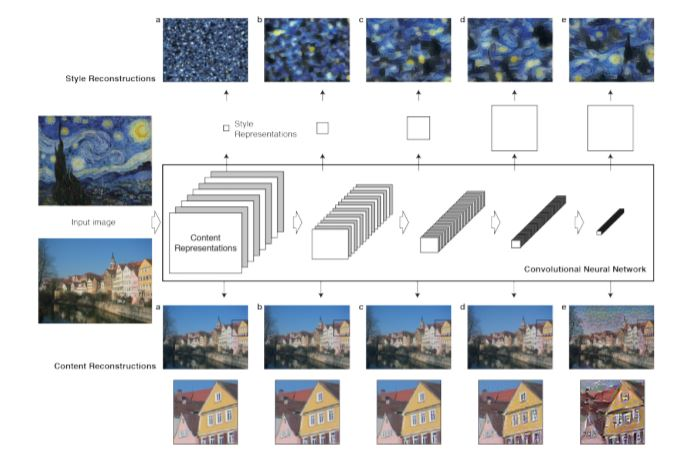
\includegraphics[width=80mm]{exp.jpg}
    \end{center}
\end{frame}

\begin{frame}
		\frametitle{Key Finding}
		The representations of content and style in the Convolutional Neural Network are separable.
\end{frame}

\begin{frame}
		\frametitle{Technical Stack}
		\setbeamertemplate{itemize items}[ball]
		\begin{itemize}
		\item Keras 
        \item Tensorflow
		\item NumPy
		\item SciPy
        \item Matplotlib
		\item Flask  
		\end{itemize}
\end{frame}

\begin{frame}
		\frametitle{Status and Statistics}
		\setbeamertemplate{itemize items}[ball]
		\begin{itemize}
		\item Project completed
        \item Total lines of code: 1122
		\item Total number of commits: 210
		\end{itemize}
\end{frame}

\begin{frame}
		\frametitle{Learnings}
		\setbeamertemplate{itemize items}[ball]
        \begin{itemize}
		\item Convolutional Neural Networks in deep learning
        \item Developing web application using HTML, CSS, JavaScript and Flask
		\item Version Control System
		\item Presentation using Beamer
		\end{itemize}
\end{frame}

\begin{frame}
		\frametitle{Difficulties Faced}
		\setbeamertemplate{itemize items}[ball]
        \begin{itemize}

				\item The program was taking lot of time to output stylized image
                \item Allocating space for user images
		\end{itemize}
\end{frame}

\begin{frame}
    \begin{center}
        \Huge Demo
    \end{center}
\end{frame}

\begin{frame}
    Collage here...
\end{frame}
\begin{frame}
    \frametitle{Future Extensions}
    \setbeamertemplate{itemize item}[ball]
    \begin{itemize}
    \item Apply neural style transfer algorithm on videos
    \item Edit photos of different formats
    \item Photo editor- image enhancement, image manipulation, crop, rotate etc
    \end{itemize}
\end{frame}

\begin{frame}
    \begin{center}  
       \Huge Thank You!
    \end{center}
\end{frame}

\end{document}
